\begin{figure*}
\center
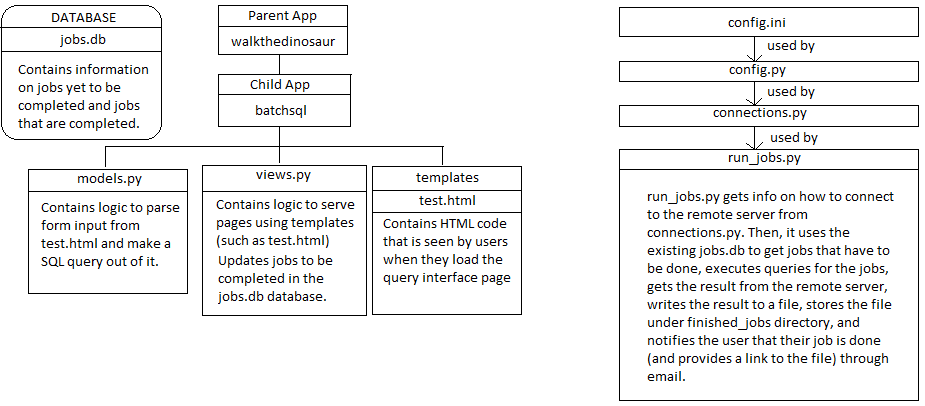
\includegraphics[width=.8\textwidth]{figs/structure}
\caption{Structure of app}
\label{fig:structure}
\end{figure*}

The application is available on github at \verb`https://github.com/gtfierro/walkthedinosaur`. The application consists of three services: the django app that parses user input and turns it into a query, a python file that executes the query, gets the result from the remote MySQL database, writes it to a file and emails the user a notification which contains a download link to the file, and a fileserver that serves files to the user. 

All the models, templates and views are stored in the batchsql folter. The python file that executes the query is called \verb`run_jobs.py`. The information to connect to the remote server and other configurations are stored in \verb`config.ini`.